\chapter{Hasil \textit{Usability Testing} Prototipe \textit{High-Fidelity} Iterasi Pertama}
\label{chpt:hasil_test_hifi1}

\large \section{Rangkuman Hasil SUS}
\normalsize

Jumlah partisipan adalah 5 orang.
Pertanyaan kuesioner SUS mengacu pada Lampiran \ref{subsec:sus}.

\begin{figure}[h]
  \centering
  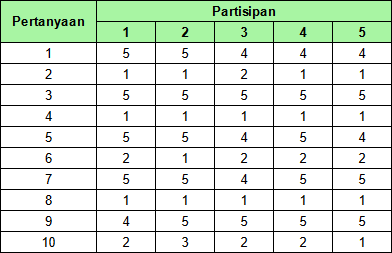
\includegraphics[width=0.7\textwidth]{hifi/chart-sus.png}
\end{figure}


\large \section{Konversi Penghitungan Skor SUS dan SEQ}
\normalsize
Berikut adalah hasil konversi perhitungan skor SUS dan skor SEQ. Daftar \textit{task} mengacu pada Lampiran \ref{chpt:skenario_hifi1}.

\begin{figure}[h]
  \centering
  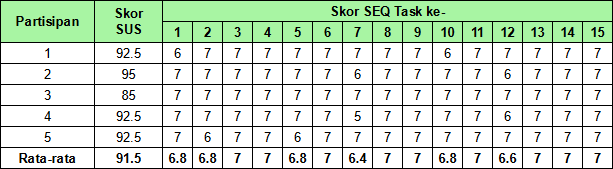
\includegraphics[width=\textwidth]{hifi/chart-sus-seq.png}
\end{figure}

\large \section{Waktu Penyelesaian Task}
\normalsize

Berikut adalah rangkuman waktu yang diperlukan setiap partisipan untuk menyelesaikan \textit{task} yang diberikan. Daftar \textit{task} mengacu pada Lampiran \ref{chpt:skenario_hifi1}.

\begin{figure}[h]
  \centering
  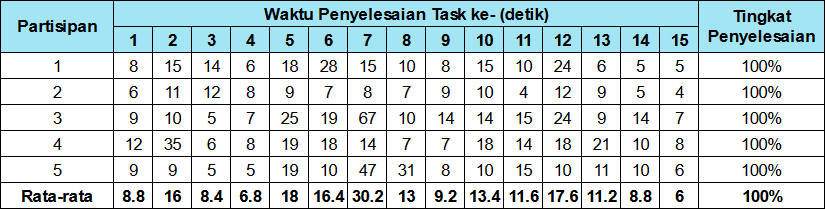
\includegraphics[width=\textwidth]{hifi/chart-penyelesaian.png}
\end{figure}

\large \section{Konversi Perhitungan Skor IMI}
\normalsize

Berikut adalah rata-rata nilai 3 sub skala \textit{Intrinsic Motivation Inventory}. Daftar pertanyaan pada setiap sub skala IMI mengacu pada Lampiran \ref{subsec:imi}.

\begin{figure}[h]
  \centering
  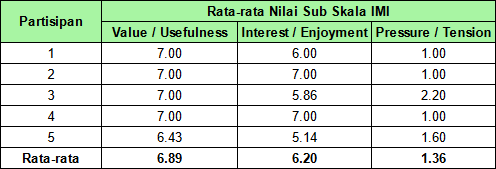
\includegraphics[width=0.95\textwidth]{hifi/chart-imi.png}
\end{figure}